\documentclass[12pt, a4paper, twoside]{article}

%% Preamble
\usepackage{umatfgspanish}
\usepackage[backend=biber]{biblatex}
\addbibresource{bibliografia.bib} 
\usepackage{subfiles}
\usepackage{blindtext}
\graphicspath{ {./images/} }



\begin{document}


%% Front Cover
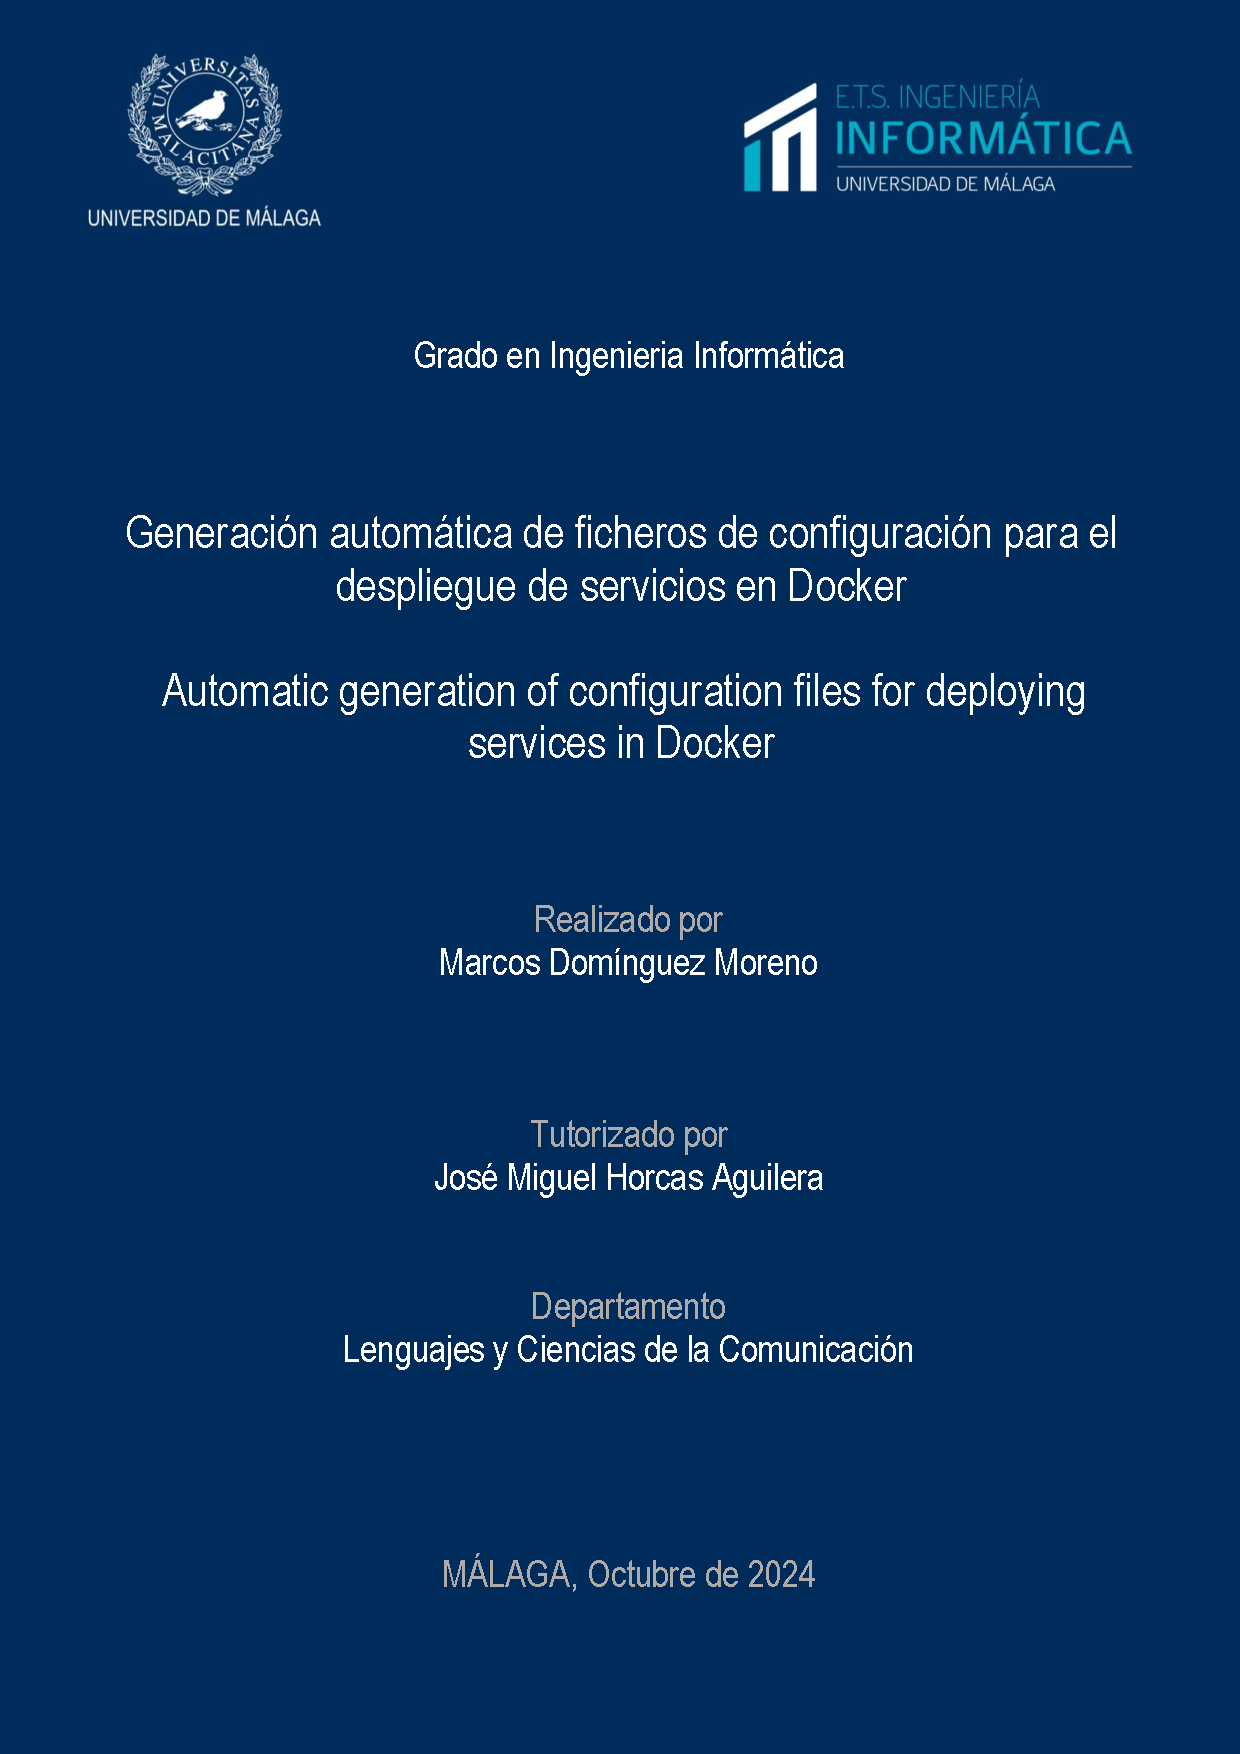
\includepdf[noautoscale=true, width=\paperwidth]{Portada-Titulo-Contraportada/cover.pdf}
\newpage

%% Title Page

\includepdf[noautoscale=true, width=\paperwidth]{Portada-Titulo-Contraportada/title.pdf}

%% Abstract
\subfile{sections/abstract}
\newpage

%% Resumen
\subfile{sections/resumen}
\newpage

% Table of Contents
\tableofcontents
\newpage








%% Introduction
\section{Introduction}

\subsection{Motivación}
Las herramientas de automatización de tareas son fundamentales en el desarrollo de software, ya que permiten mejorar la eficiencia, la calidad y la consistencia en la producción de código.
Al relegar tareas repetitivas y propensas a errores a herramientas automatizadas, los desarrolladores pueden centrarse en tareas más creativas y de mayor valor añadido.
Parte del ciclo de vida en un desarrollo de software implica la configuración y el despliegue de servicios en entornos de producción y desarrollo.
La configuracion y despliegue requiere de la creación de archivos de configuración específicos, como los archivos Dockerfile y .dockerignore, que definen cómo se construye y se ejecuta una aplicación en un contenedor de Docker.
En el contexto de la tecnología de contenedores, Docker se ha convertido en una de las plataformas más populares para la creación, el despliegue y la gestión de aplicaciones en entornos contenerizados. 
Sin embargo, la configuración de servicios en Docker puede ser una tarea compleja y propensa a errores, especialmente cuando se manejan múltiples servicios y configuraciones personalizadas.
La motivación para realizar este proyecto surge de la necesidad de simplificar y automatizar el proceso de generación de archivos de configuración para el despliegue de servicios en Docker. 
En la actualidad, la creación manual de estos archivos dockerfile puede ser una tarea tediosa y propensa a errores al no conocer el usuario de toda la informacion necesaria para la correcta configuracion de los servicios, 
Al desarrollar una herramienta que automatice este proceso, 
se busca mejorar la eficiencia y la precisión en la configuración de entornos de contenedores, facilitando así el trabajo de desarrollo y administracion. 

\subsection{Objetivos}
El objetivo principal de este proyecto es desarrollar una herramienta que permita la generación automática de archivos de configuración para el despliegue de servicios en Docker.

\subsection{Resultados Esperados}
Dada la gran cantidad de opciones de configuración disponibles en para la generacion de ficheros de configuracion como puedes ser dockerfile..., el desarrollo de esta herramienta presenta varios desafíos técnicos y conceptuales.
El primero de ellos es la magnitud de las opciones de configuración disponibles, que pueden variar en función de las necesidades y los requisitos de cada servicio.
dar una covertura a todos los escenarios posibles es una tarea inabarcable, por lo que se ha optado por centrarse en los casos de uso más comunes y en las configuraciones más utilizadas en la práctica.
Sin embargo se espera que la herramienta sea lo suficientemente flexible y extensible como para permitir la incorporación de nuevas plantillas y configuraciones en el futuro.


\subsection{Estructura del documento}
Por definir










%% Estado del Arte 
\section{Estado del Arte}
Para la realización de este proyecto se ha realizado un estudio del estado del arte en el ámbito de la generación de archivos de configuración para el despliegue de servicios en Docker.
En este apartado se presentan las principales herramientas y tecnologías disponibles en la actualidad, así como las tendencias y los enfoques más comunes en la configuración de servicios en entornos de contenedores.
\subsection{Contenedores}
Los contenedores son paquetes ligeros que incluyen el código de las aplicaciones junto con sus dependencias, como versiones concretas de entornos de ejecución de ciertos lenguajes de programación y bibliotecas indispensables para ejecutar los servicios de software.
\subsection{imagenes}
Las imágenes de contenedores son plantillas de solo lectura que contienen el código de la aplicación, las bibliotecas, las dependencias y otros archivos necesarios para ejecutar un contenedor.
\subsection{Docker}
Docker es un proyecto de código abierto que automatiza el despliegue de aplicaciones dentro de contenedores de software, proporcionando una capa adicional de abstracción y automatización de virtualización de aplicaciones en múltiples sistemas operativos
Docker es una plataforma de código abierto que permite a los desarrolladores crear, desplegar y ejecutar aplicaciones en contenedores. 
\subsubsection{Dockerfile}
El archivo Dockerfile es un archivo de texto que contiene una serie de instrucciones que Docker utilizará para construir una imagen de contenedor.
Usualmente la construccion de un archivo de configuracion se realiza a partir de una imagen base, que puede ser una imagen oficial de Docker o una imagen personalizada creada por el usuario.
A dicha imagen se añaden las instrucciones necesarias para instalar las dependencias y configurar el entorno de ejecución de la aplicación, lo que viene a representar el contenido de un archivo Dockerfile.
\subsubsection{Buenas Prácticas}
Para la creacion de los ficheros dockerfile es recomendable seguir una serie de buenas practicas para garantizar la eficiencia y la seguridad en el despliegue de servicios en Docker.
Estas practicas se recojen en la documentacion oficial de Docker y en guias de buenas practicas de la comunidad de desarrolladores.
\subsection{Alternativas Actualmente Disponibles}
\subsubsection{Docker init , Docker Extension vscode1}
\subsubsection{https://magickpen.com/templates/128/}
\subsubsection{https://phpdocker.io/}
\blindtext

\subsection{Conclusiones}
\blindtext

\subsection{Que se aporta en este contexto:}
\blindtext













%% Tecnologías Empleadas
\section{Tecnologías Empleadas}

\subsection{UVL}
\subsubsection{Feature Models}

\subsection{Docker}
\subsubsection{Docker Desktop}

\subsection{Node}
\subsection{Angular}
\subsubsection{Angular Material}
\subsubsection{Monaco Editor}
\subsubsection{ngx-json-viewer}

\subsection{Nginx}
\subsubsection{Reverse Proxy}
\subsubsection{Web Server}

\subsection{Python}
\subsubsection{Flask}
\subsubsection{Pypi}

\subsection{Git}
\subsection{GitHub}
\subsubsection{GitHub Public Api}
\blindtext

\subsection{Visual Studio Code}
\subsubsection{UVLS extension}
EXTENSIONES VISUAL ESTUDIO
	-UVLS https://github.com/Universal-Variability-Language/uvl-lsp
	-Docker
	-Flama https://marketplace.visualstudio.com/items?itemName=diversolab.flamapy
	-Graphiz Inetractive Preview https://marketplace.visualstudio.com/items?itemName=tintinweb.graphviz-interactive-preview
	-Latex Worshop
	-Pylance
	-Python
	-Python Debugger
	-Better Jinja






%% Metodología
\section{Metodologia del trabajo. (Fases) Implementación:}
\subsection{Enfoque/Procedimiento/Justificación/Limitaciones}
\subsection{Estudio del Estado del Arte :}
\subsection{Investigación opciones de configuración para Docker}
\subsection{Requisitios de la aplicación }
\subsection{Desarrollo Modelos plantillas dockerfile y dockerignore …}
\subsection{Desarrollo del la aplicación de uvengine }
\subsection{Desarrollo de la web}
\subsection{Desarrollo de los servicios de backend}
\subsection{Elaboración de la guía de uso}
\subsection{Elaboración de un manual de instalación}
\subsection{Elaboración de la memoria}


%% Arquitectura y Modelado del sistema
\section{Arquitectura y Modelado del sistema }
\subsection{Vision general de la arquitectura }
\subsection{Arquitectura de backend}
\subsection{Arquitectura de Frontend}


%% Despliegue de la aplicación
\section{Despliegue de la aplicación  }
\subsection{ Despliegue local }
\subsection{ Despliegue en la nube }



%% Resultados
\section{Resultados}
\subsection{Resultados Obtenidos}
\subsection{Viabilidad del proyecto}


%% Conclusiones
\section{Conclusiones y líneas Futuras }
\subsection{Conclusion Personal,}
\subsection{Conclusiones del Desarrollo del proyecto}
\subsection{Contribuciones / Aplicaciones Prácticas}
\subsection{Desarrollo de nuevas plantillas }
\subsection{Continuación en el desarrollo de plantillas ya existentes}
\subsection{Mejorar la experiencia del usuario }








%%%% Sections
%%\section{One \\}
%%
%%\subsection{Motivation}
%%    \blindtext[2]
%%    
%%    \begin{figure}[ht]
%%      \centering
%%        
\includegraphics[width=0.5\textwidth]{xp}
%%      \caption{A diagram showing the iterations of extreme programming.}
%%    \end{figure}
%%    
%%    \blindtext[4]
%%
%%\section{Two \\}
%%    \blindmathpaper






% Imprimir la bibliografía
\printbibliography




%% Bibliografia
%%\begin{thebibliography}{9}
%%    \bibitem{latexcompanion} 
%%    Michel Goossens, Frank Mittelbach, and Alexander Samarin. 
%%    \textit{The \LaTeX\ Companion}. 
%%    Addison-Wesley, Reading, Massachusetts, 1993.
%%    
%%    \bibitem{einstein} 
%%    Albert Einstein. 
%%    \textit{Zur Elektrodynamik bewegter K{\"o}rper}. (German) 
%%    [\textit{On the electrodynamics of moving bodies}]. 
%%    Annalen der Physik, 322(10):891–921, 1905.
%%\end{thebibliography}




%%\end{document}















%% Apendices
\begin{umaappendices}
    \section{Manual de \\ Instalación}
    \section{Manual de Uso}
\end{umaappendices}


%% Back Cover

\includepdf[noautoscale=true, width=\paperwidth]{Portada-Titulo-Contraportada/backcover.pdf}
\end{document}



\end{document}